% Created by tikzDevice version 0.12.3.2 on 2022-02-18 18:11:57
% !TEX encoding = UTF-8 Unicode
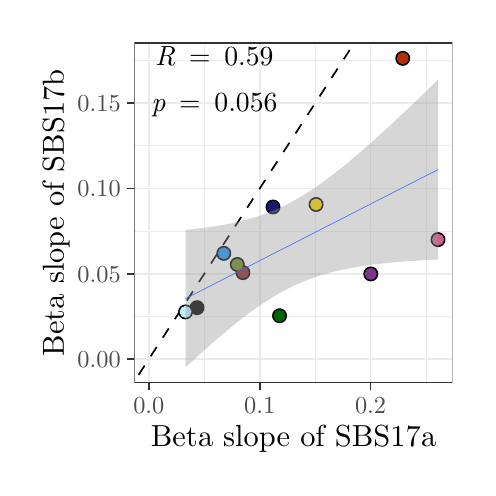
\begin{tikzpicture}[x=1pt,y=1pt]
\definecolor{fillColor}{RGB}{255,255,255}
\path[use as bounding box,fill=fillColor,fill opacity=0.00] (0,0) rectangle (158.99,158.99);
\begin{scope}
\path[clip] (  0.00,  0.00) rectangle (158.99,158.99);
\definecolor{drawColor}{RGB}{255,255,255}
\definecolor{fillColor}{RGB}{255,255,255}

\path[draw=drawColor,line width= 0.6pt,line join=round,line cap=round,fill=fillColor] (  0.00,  0.00) rectangle (158.99,158.99);
\end{scope}
\begin{scope}
\path[clip] ( 38.56, 30.69) rectangle (153.49,153.49);
\definecolor{fillColor}{RGB}{255,255,255}

\path[fill=fillColor] ( 38.56, 30.69) rectangle (153.49,153.49);
\definecolor{drawColor}{gray}{0.92}

\path[draw=drawColor,line width= 0.3pt,line join=round] ( 38.56, 54.64) --
	(153.49, 54.64);

\path[draw=drawColor,line width= 0.3pt,line join=round] ( 38.56, 85.46) --
	(153.49, 85.46);

\path[draw=drawColor,line width= 0.3pt,line join=round] ( 38.56,116.29) --
	(153.49,116.29);

\path[draw=drawColor,line width= 0.3pt,line join=round] ( 38.56,147.12) --
	(153.49,147.12);

\path[draw=drawColor,line width= 0.3pt,line join=round] ( 63.81, 30.69) --
	( 63.81,153.49);

\path[draw=drawColor,line width= 0.3pt,line join=round] (103.88, 30.69) --
	(103.88,153.49);

\path[draw=drawColor,line width= 0.3pt,line join=round] (143.95, 30.69) --
	(143.95,153.49);

\path[draw=drawColor,line width= 0.6pt,line join=round] ( 38.56, 39.22) --
	(153.49, 39.22);

\path[draw=drawColor,line width= 0.6pt,line join=round] ( 38.56, 70.05) --
	(153.49, 70.05);

\path[draw=drawColor,line width= 0.6pt,line join=round] ( 38.56,100.88) --
	(153.49,100.88);

\path[draw=drawColor,line width= 0.6pt,line join=round] ( 38.56,131.71) --
	(153.49,131.71);

\path[draw=drawColor,line width= 0.6pt,line join=round] ( 43.78, 30.69) --
	( 43.78,153.49);

\path[draw=drawColor,line width= 0.6pt,line join=round] ( 83.85, 30.69) --
	( 83.85,153.49);

\path[draw=drawColor,line width= 0.6pt,line join=round] (123.92, 30.69) --
	(123.92,153.49);
\definecolor{drawColor}{RGB}{0,0,0}

\path[draw=drawColor,line width= 0.6pt,dash pattern=on 4pt off 4pt ,line join=round] ( 18.29,  0.00) -- (121.62,158.99);
\definecolor{fillColor}{RGB}{0,0,0}

\path[draw=drawColor,line width= 0.4pt,line join=round,line cap=round,fill=fillColor] (104.21, 95.10) circle (  2.50);

\path[draw=drawColor,line width= 0.4pt,line join=round,line cap=round,fill=fillColor] (148.27, 82.40) circle (  2.50);

\path[draw=drawColor,line width= 0.4pt,line join=round,line cap=round,fill=fillColor] ( 88.65, 94.19) circle (  2.50);

\path[draw=drawColor,line width= 0.4pt,line join=round,line cap=round,fill=fillColor] ( 70.86, 77.44) circle (  2.50);

\path[draw=drawColor,line width= 0.4pt,line join=round,line cap=round,fill=fillColor] ( 77.78, 70.47) circle (  2.50);

\path[draw=drawColor,line width= 0.4pt,line join=round,line cap=round,fill=fillColor] (135.54,147.91) circle (  2.50);

\path[draw=drawColor,line width= 0.4pt,line join=round,line cap=round,fill=fillColor] ( 91.02, 54.90) circle (  2.50);

\path[draw=drawColor,line width= 0.4pt,line join=round,line cap=round,fill=fillColor] ( 75.74, 73.42) circle (  2.50);

\path[draw=drawColor,line width= 0.4pt,line join=round,line cap=round,fill=fillColor] (123.98, 70.01) circle (  2.50);

\path[draw=drawColor,line width= 0.4pt,line join=round,line cap=round,fill=fillColor] ( 61.20, 57.81) circle (  2.50);

\path[draw=drawColor,line width= 0.4pt,line join=round,line cap=round,fill=fillColor] ( 57.04, 56.28) circle (  2.50);
\definecolor{drawColor}{RGB}{255,215,0}
\definecolor{fillColor}{RGB}{255,215,0}

\path[draw=drawColor,line width= 0.4pt,line join=round,line cap=round,fill=fillColor] (104.21, 95.10) circle (  1.96);
\definecolor{drawColor}{RGB}{205,96,144}
\definecolor{fillColor}{RGB}{205,96,144}

\path[draw=drawColor,line width= 0.4pt,line join=round,line cap=round,fill=fillColor] (148.27, 82.40) circle (  1.96);
\definecolor{drawColor}{RGB}{25,25,112}
\definecolor{fillColor}{RGB}{25,25,112}

\path[draw=drawColor,line width= 0.4pt,line join=round,line cap=round,fill=fillColor] ( 88.65, 94.19) circle (  1.96);
\definecolor{drawColor}{RGB}{30,144,255}
\definecolor{fillColor}{RGB}{30,144,255}

\path[draw=drawColor,line width= 0.4pt,line join=round,line cap=round,fill=fillColor] ( 70.86, 77.44) circle (  1.96);
\definecolor{drawColor}{RGB}{139,35,35}
\definecolor{fillColor}{RGB}{139,35,35}

\path[draw=drawColor,line width= 0.4pt,line join=round,line cap=round,fill=fillColor] ( 77.78, 70.47) circle (  1.96);
\definecolor{drawColor}{RGB}{179,47,11}
\definecolor{fillColor}{RGB}{179,47,11}

\path[draw=drawColor,line width= 0.4pt,line join=round,line cap=round,fill=fillColor] (135.54,147.91) circle (  1.96);
\definecolor{drawColor}{RGB}{0,100,0}
\definecolor{fillColor}{RGB}{0,100,0}

\path[draw=drawColor,line width= 0.4pt,line join=round,line cap=round,fill=fillColor] ( 91.02, 54.90) circle (  1.96);
\definecolor{drawColor}{RGB}{105,139,34}
\definecolor{fillColor}{RGB}{105,139,34}

\path[draw=drawColor,line width= 0.4pt,line join=round,line cap=round,fill=fillColor] ( 75.74, 73.42) circle (  1.96);
\definecolor{drawColor}{RGB}{122,55,139}
\definecolor{fillColor}{RGB}{122,55,139}

\path[draw=drawColor,line width= 0.4pt,line join=round,line cap=round,fill=fillColor] (123.98, 70.01) circle (  1.96);
\definecolor{drawColor}{RGB}{0,0,0}
\definecolor{fillColor}{RGB}{0,0,0}

\path[draw=drawColor,line width= 0.4pt,line join=round,line cap=round,fill=fillColor] ( 61.20, 57.81) circle (  1.96);
\definecolor{drawColor}{RGB}{191,239,255}
\definecolor{fillColor}{RGB}{191,239,255}

\path[draw=drawColor,line width= 0.4pt,line join=round,line cap=round,fill=fillColor] ( 57.04, 56.28) circle (  1.96);
\definecolor{fillColor}{RGB}{153,153,153}

\path[fill=fillColor,fill opacity=0.40] ( 57.04, 85.92) --
	( 58.19, 86.03) --
	( 59.35, 86.15) --
	( 60.50, 86.28) --
	( 61.65, 86.41) --
	( 62.81, 86.55) --
	( 63.96, 86.70) --
	( 65.12, 86.86) --
	( 66.27, 87.02) --
	( 67.43, 87.20) --
	( 68.58, 87.38) --
	( 69.74, 87.57) --
	( 70.89, 87.78) --
	( 72.05, 87.99) --
	( 73.20, 88.22) --
	( 74.36, 88.46) --
	( 75.51, 88.72) --
	( 76.67, 88.99) --
	( 77.82, 89.27) --
	( 78.98, 89.58) --
	( 80.13, 89.89) --
	( 81.29, 90.23) --
	( 82.44, 90.58) --
	( 83.60, 90.96) --
	( 84.75, 91.35) --
	( 85.91, 91.77) --
	( 87.06, 92.20) --
	( 88.22, 92.66) --
	( 89.37, 93.15) --
	( 90.53, 93.65) --
	( 91.68, 94.18) --
	( 92.84, 94.73) --
	( 93.99, 95.31) --
	( 95.15, 95.91) --
	( 96.30, 96.54) --
	( 97.46, 97.19) --
	( 98.61, 97.86) --
	( 99.77, 98.56) --
	(100.92, 99.28) --
	(102.08,100.02) --
	(103.23,100.78) --
	(104.38,101.57) --
	(105.54,102.37) --
	(106.69,103.20) --
	(107.85,104.04) --
	(109.00,104.90) --
	(110.16,105.78) --
	(111.31,106.67) --
	(112.47,107.58) --
	(113.62,108.50) --
	(114.78,109.44) --
	(115.93,110.39) --
	(117.09,111.36) --
	(118.24,112.33) --
	(119.40,113.32) --
	(120.55,114.31) --
	(121.71,115.32) --
	(122.86,116.33) --
	(124.02,117.36) --
	(125.17,118.39) --
	(126.33,119.43) --
	(127.48,120.47) --
	(128.64,121.53) --
	(129.79,122.59) --
	(130.95,123.65) --
	(132.10,124.73) --
	(133.26,125.80) --
	(134.41,126.89) --
	(135.57,127.97) --
	(136.72,129.07) --
	(137.88,130.16) --
	(139.03,131.26) --
	(140.19,132.37) --
	(141.34,133.47) --
	(142.50,134.58) --
	(143.65,135.70) --
	(144.80,136.82) --
	(145.96,137.94) --
	(147.11,139.06) --
	(148.27,140.19) --
	(148.27, 75.23) --
	(147.11, 75.17) --
	(145.96, 75.12) --
	(144.80, 75.06) --
	(143.65, 75.00) --
	(142.50, 74.93) --
	(141.34, 74.86) --
	(140.19, 74.79) --
	(139.03, 74.71) --
	(137.88, 74.63) --
	(136.72, 74.55) --
	(135.57, 74.46) --
	(134.41, 74.37) --
	(133.26, 74.27) --
	(132.10, 74.17) --
	(130.95, 74.06) --
	(129.79, 73.95) --
	(128.64, 73.83) --
	(127.48, 73.70) --
	(126.33, 73.57) --
	(125.17, 73.43) --
	(124.02, 73.28) --
	(122.86, 73.12) --
	(121.71, 72.96) --
	(120.55, 72.78) --
	(119.40, 72.60) --
	(118.24, 72.40) --
	(117.09, 72.20) --
	(115.93, 71.98) --
	(114.78, 71.75) --
	(113.62, 71.51) --
	(112.47, 71.25) --
	(111.31, 70.98) --
	(110.16, 70.70) --
	(109.00, 70.39) --
	(107.85, 70.07) --
	(106.69, 69.74) --
	(105.54, 69.38) --
	(104.38, 69.01) --
	(103.23, 68.61) --
	(102.08, 68.19) --
	(100.92, 67.76) --
	( 99.77, 67.29) --
	( 98.61, 66.81) --
	( 97.46, 66.30) --
	( 96.30, 65.77) --
	( 95.15, 65.22) --
	( 93.99, 64.64) --
	( 92.84, 64.04) --
	( 91.68, 63.41) --
	( 90.53, 62.76) --
	( 89.37, 62.09) --
	( 88.22, 61.39) --
	( 87.06, 60.67) --
	( 85.91, 59.92) --
	( 84.75, 59.16) --
	( 83.60, 58.37) --
	( 82.44, 57.57) --
	( 81.29, 56.74) --
	( 80.13, 55.90) --
	( 78.98, 55.04) --
	( 77.82, 54.16) --
	( 76.67, 53.26) --
	( 75.51, 52.35) --
	( 74.36, 51.43) --
	( 73.20, 50.49) --
	( 72.05, 49.54) --
	( 70.89, 48.57) --
	( 69.74, 47.60) --
	( 68.58, 46.61) --
	( 67.43, 45.61) --
	( 66.27, 44.61) --
	( 65.12, 43.59) --
	( 63.96, 42.57) --
	( 62.81, 41.54) --
	( 61.65, 40.50) --
	( 60.50, 39.45) --
	( 59.35, 38.39) --
	( 58.19, 37.33) --
	( 57.04, 36.27) --
	cycle;

\path[] ( 57.04, 85.92) --
	( 58.19, 86.03) --
	( 59.35, 86.15) --
	( 60.50, 86.28) --
	( 61.65, 86.41) --
	( 62.81, 86.55) --
	( 63.96, 86.70) --
	( 65.12, 86.86) --
	( 66.27, 87.02) --
	( 67.43, 87.20) --
	( 68.58, 87.38) --
	( 69.74, 87.57) --
	( 70.89, 87.78) --
	( 72.05, 87.99) --
	( 73.20, 88.22) --
	( 74.36, 88.46) --
	( 75.51, 88.72) --
	( 76.67, 88.99) --
	( 77.82, 89.27) --
	( 78.98, 89.58) --
	( 80.13, 89.89) --
	( 81.29, 90.23) --
	( 82.44, 90.58) --
	( 83.60, 90.96) --
	( 84.75, 91.35) --
	( 85.91, 91.77) --
	( 87.06, 92.20) --
	( 88.22, 92.66) --
	( 89.37, 93.15) --
	( 90.53, 93.65) --
	( 91.68, 94.18) --
	( 92.84, 94.73) --
	( 93.99, 95.31) --
	( 95.15, 95.91) --
	( 96.30, 96.54) --
	( 97.46, 97.19) --
	( 98.61, 97.86) --
	( 99.77, 98.56) --
	(100.92, 99.28) --
	(102.08,100.02) --
	(103.23,100.78) --
	(104.38,101.57) --
	(105.54,102.37) --
	(106.69,103.20) --
	(107.85,104.04) --
	(109.00,104.90) --
	(110.16,105.78) --
	(111.31,106.67) --
	(112.47,107.58) --
	(113.62,108.50) --
	(114.78,109.44) --
	(115.93,110.39) --
	(117.09,111.36) --
	(118.24,112.33) --
	(119.40,113.32) --
	(120.55,114.31) --
	(121.71,115.32) --
	(122.86,116.33) --
	(124.02,117.36) --
	(125.17,118.39) --
	(126.33,119.43) --
	(127.48,120.47) --
	(128.64,121.53) --
	(129.79,122.59) --
	(130.95,123.65) --
	(132.10,124.73) --
	(133.26,125.80) --
	(134.41,126.89) --
	(135.57,127.97) --
	(136.72,129.07) --
	(137.88,130.16) --
	(139.03,131.26) --
	(140.19,132.37) --
	(141.34,133.47) --
	(142.50,134.58) --
	(143.65,135.70) --
	(144.80,136.82) --
	(145.96,137.94) --
	(147.11,139.06) --
	(148.27,140.19);

\path[] (148.27, 75.23) --
	(147.11, 75.17) --
	(145.96, 75.12) --
	(144.80, 75.06) --
	(143.65, 75.00) --
	(142.50, 74.93) --
	(141.34, 74.86) --
	(140.19, 74.79) --
	(139.03, 74.71) --
	(137.88, 74.63) --
	(136.72, 74.55) --
	(135.57, 74.46) --
	(134.41, 74.37) --
	(133.26, 74.27) --
	(132.10, 74.17) --
	(130.95, 74.06) --
	(129.79, 73.95) --
	(128.64, 73.83) --
	(127.48, 73.70) --
	(126.33, 73.57) --
	(125.17, 73.43) --
	(124.02, 73.28) --
	(122.86, 73.12) --
	(121.71, 72.96) --
	(120.55, 72.78) --
	(119.40, 72.60) --
	(118.24, 72.40) --
	(117.09, 72.20) --
	(115.93, 71.98) --
	(114.78, 71.75) --
	(113.62, 71.51) --
	(112.47, 71.25) --
	(111.31, 70.98) --
	(110.16, 70.70) --
	(109.00, 70.39) --
	(107.85, 70.07) --
	(106.69, 69.74) --
	(105.54, 69.38) --
	(104.38, 69.01) --
	(103.23, 68.61) --
	(102.08, 68.19) --
	(100.92, 67.76) --
	( 99.77, 67.29) --
	( 98.61, 66.81) --
	( 97.46, 66.30) --
	( 96.30, 65.77) --
	( 95.15, 65.22) --
	( 93.99, 64.64) --
	( 92.84, 64.04) --
	( 91.68, 63.41) --
	( 90.53, 62.76) --
	( 89.37, 62.09) --
	( 88.22, 61.39) --
	( 87.06, 60.67) --
	( 85.91, 59.92) --
	( 84.75, 59.16) --
	( 83.60, 58.37) --
	( 82.44, 57.57) --
	( 81.29, 56.74) --
	( 80.13, 55.90) --
	( 78.98, 55.04) --
	( 77.82, 54.16) --
	( 76.67, 53.26) --
	( 75.51, 52.35) --
	( 74.36, 51.43) --
	( 73.20, 50.49) --
	( 72.05, 49.54) --
	( 70.89, 48.57) --
	( 69.74, 47.60) --
	( 68.58, 46.61) --
	( 67.43, 45.61) --
	( 66.27, 44.61) --
	( 65.12, 43.59) --
	( 63.96, 42.57) --
	( 62.81, 41.54) --
	( 61.65, 40.50) --
	( 60.50, 39.45) --
	( 59.35, 38.39) --
	( 58.19, 37.33) --
	( 57.04, 36.27);
\definecolor{drawColor}{RGB}{51,102,255}

\path[draw=drawColor,line width= 0.2pt,line join=round] ( 57.04, 61.09) --
	( 58.19, 61.68) --
	( 59.35, 62.27) --
	( 60.50, 62.86) --
	( 61.65, 63.45) --
	( 62.81, 64.04) --
	( 63.96, 64.63) --
	( 65.12, 65.22) --
	( 66.27, 65.81) --
	( 67.43, 66.40) --
	( 68.58, 66.99) --
	( 69.74, 67.59) --
	( 70.89, 68.18) --
	( 72.05, 68.77) --
	( 73.20, 69.36) --
	( 74.36, 69.95) --
	( 75.51, 70.54) --
	( 76.67, 71.13) --
	( 77.82, 71.72) --
	( 78.98, 72.31) --
	( 80.13, 72.90) --
	( 81.29, 73.49) --
	( 82.44, 74.08) --
	( 83.60, 74.67) --
	( 84.75, 75.26) --
	( 85.91, 75.85) --
	( 87.06, 76.44) --
	( 88.22, 77.03) --
	( 89.37, 77.62) --
	( 90.53, 78.21) --
	( 91.68, 78.80) --
	( 92.84, 79.39) --
	( 93.99, 79.98) --
	( 95.15, 80.57) --
	( 96.30, 81.16) --
	( 97.46, 81.75) --
	( 98.61, 82.34) --
	( 99.77, 82.93) --
	(100.92, 83.52) --
	(102.08, 84.11) --
	(103.23, 84.70) --
	(104.38, 85.29) --
	(105.54, 85.88) --
	(106.69, 86.47) --
	(107.85, 87.06) --
	(109.00, 87.65) --
	(110.16, 88.24) --
	(111.31, 88.83) --
	(112.47, 89.42) --
	(113.62, 90.01) --
	(114.78, 90.60) --
	(115.93, 91.19) --
	(117.09, 91.78) --
	(118.24, 92.37) --
	(119.40, 92.96) --
	(120.55, 93.55) --
	(121.71, 94.14) --
	(122.86, 94.73) --
	(124.02, 95.32) --
	(125.17, 95.91) --
	(126.33, 96.50) --
	(127.48, 97.09) --
	(128.64, 97.68) --
	(129.79, 98.27) --
	(130.95, 98.86) --
	(132.10, 99.45) --
	(133.26,100.04) --
	(134.41,100.63) --
	(135.57,101.22) --
	(136.72,101.81) --
	(137.88,102.40) --
	(139.03,102.99) --
	(140.19,103.58) --
	(141.34,104.17) --
	(142.50,104.76) --
	(143.65,105.35) --
	(144.80,105.94) --
	(145.96,106.53) --
	(147.11,107.12) --
	(148.27,107.71);
\definecolor{drawColor}{RGB}{0,0,0}

\node[text=drawColor,anchor=base west,inner sep=0pt, outer sep=0pt, scale=  1.00] at ( 46.09,145.35) {\itshape R};

\node[text=drawColor,anchor=base west,inner sep=0pt, outer sep=0pt, scale=  1.00] at ( 53.35,145.35) { };

\node[text=drawColor,anchor=base west,inner sep=0pt, outer sep=0pt, scale=  1.00] at ( 58.33,145.35) {=};

\node[text=drawColor,anchor=base west,inner sep=0pt, outer sep=0pt, scale=  1.00] at ( 66.07,145.35) { };

\node[text=drawColor,anchor=base west,inner sep=0pt, outer sep=0pt, scale=  1.00] at ( 71.05,145.35) {0.59};

\node[text=drawColor,anchor=base west,inner sep=0pt, outer sep=0pt, scale=  1.00] at ( 44.69,128.52) {\itshape p};

\node[text=drawColor,anchor=base west,inner sep=0pt, outer sep=0pt, scale=  1.00] at ( 49.78,128.52) { };

\node[text=drawColor,anchor=base west,inner sep=0pt, outer sep=0pt, scale=  1.00] at ( 54.76,128.52) {=};

\node[text=drawColor,anchor=base west,inner sep=0pt, outer sep=0pt, scale=  1.00] at ( 62.50,128.52) { };

\node[text=drawColor,anchor=base west,inner sep=0pt, outer sep=0pt, scale=  1.00] at ( 67.48,128.52) {0.056};
\definecolor{drawColor}{gray}{0.20}

\path[draw=drawColor,line width= 0.6pt,line join=round,line cap=round] ( 38.56, 30.69) rectangle (153.49,153.49);
\end{scope}
\begin{scope}
\path[clip] (  0.00,  0.00) rectangle (158.99,158.99);
\definecolor{drawColor}{gray}{0.30}

\node[text=drawColor,anchor=base east,inner sep=0pt, outer sep=0pt, scale=  0.88] at ( 33.61, 36.19) {0.00};

\node[text=drawColor,anchor=base east,inner sep=0pt, outer sep=0pt, scale=  0.88] at ( 33.61, 67.02) {0.05};

\node[text=drawColor,anchor=base east,inner sep=0pt, outer sep=0pt, scale=  0.88] at ( 33.61, 97.85) {0.10};

\node[text=drawColor,anchor=base east,inner sep=0pt, outer sep=0pt, scale=  0.88] at ( 33.61,128.68) {0.15};
\end{scope}
\begin{scope}
\path[clip] (  0.00,  0.00) rectangle (158.99,158.99);
\definecolor{drawColor}{gray}{0.20}

\path[draw=drawColor,line width= 0.6pt,line join=round] ( 35.81, 39.22) --
	( 38.56, 39.22);

\path[draw=drawColor,line width= 0.6pt,line join=round] ( 35.81, 70.05) --
	( 38.56, 70.05);

\path[draw=drawColor,line width= 0.6pt,line join=round] ( 35.81,100.88) --
	( 38.56,100.88);

\path[draw=drawColor,line width= 0.6pt,line join=round] ( 35.81,131.71) --
	( 38.56,131.71);
\end{scope}
\begin{scope}
\path[clip] (  0.00,  0.00) rectangle (158.99,158.99);
\definecolor{drawColor}{gray}{0.20}

\path[draw=drawColor,line width= 0.6pt,line join=round] ( 43.78, 27.94) --
	( 43.78, 30.69);

\path[draw=drawColor,line width= 0.6pt,line join=round] ( 83.85, 27.94) --
	( 83.85, 30.69);

\path[draw=drawColor,line width= 0.6pt,line join=round] (123.92, 27.94) --
	(123.92, 30.69);
\end{scope}
\begin{scope}
\path[clip] (  0.00,  0.00) rectangle (158.99,158.99);
\definecolor{drawColor}{gray}{0.30}

\node[text=drawColor,anchor=base,inner sep=0pt, outer sep=0pt, scale=  0.88] at ( 43.78, 19.68) {0.0};

\node[text=drawColor,anchor=base,inner sep=0pt, outer sep=0pt, scale=  0.88] at ( 83.85, 19.68) {0.1};

\node[text=drawColor,anchor=base,inner sep=0pt, outer sep=0pt, scale=  0.88] at (123.92, 19.68) {0.2};
\end{scope}
\begin{scope}
\path[clip] (  0.00,  0.00) rectangle (158.99,158.99);
\definecolor{drawColor}{RGB}{0,0,0}

\node[text=drawColor,anchor=base,inner sep=0pt, outer sep=0pt, scale=  1.10] at ( 96.02,  7.64) {Beta slope of SBS17a};
\end{scope}
\begin{scope}
\path[clip] (  0.00,  0.00) rectangle (158.99,158.99);
\definecolor{drawColor}{RGB}{0,0,0}

\node[text=drawColor,rotate= 90.00,anchor=base,inner sep=0pt, outer sep=0pt, scale=  1.10] at ( 13.08, 92.09) {Beta slope of SBS17b};
\end{scope}
\end{tikzpicture}
